\section{九九乘法表-兩排}
印出九九乘法表,其輸出如下圖所示。
\begin{figure}[H]
	\centering
	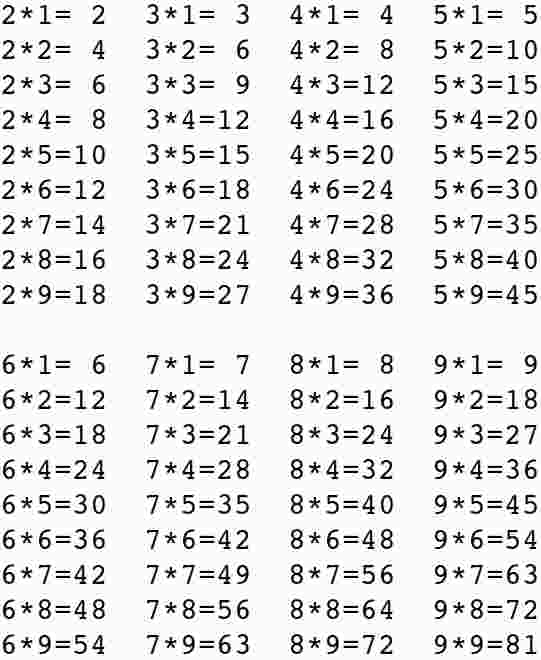
\includegraphics[height=12cm]{../solutions/fig/JA007fig}
\end{figure}

\subsection{解題思惟}
可以想成輸出兩個大群組的九九乘法表,當輸出第r (r=0, 1) 個群組時,
``被乘數"$=j+r\times4.$ (j=2, 3, 4, 5)。
			
\subsection{程式碼}
\begin{cppcode}
#include <cstdio>

int main()
{
	for (int r=0; r<2; r++) { //兩個群組
		for (int i=1; i<=9; i++) { //第i列的乘數是i
			for(int j=2; j<=5; j++) { //被乘數=j+r*4
				printf("%d*%d=%2d  ", j+r*4, i, i*(j+r*4));
			}
			printf("\n");
		}
		printf("\n");
	}
	return 0;
}
\end{cppcode}
